\subsubsection{\texttt{RF-9}: visualización de un curso y sus ejercicios}
\label{subsec:rf9}

Una vez autenticados en \textit{VSCode4Teaching} (\referenciaConTT{subsec:rf1}{RF-1.1}), los estudiantes visualizan una pantalla principal o \textit{dashboard} en el que se muestran los cursos en los que están matriculados, tal como se desarrolla en el requisito \referenciaConTT{subsec:rf1}{RF-1.2}. En esta pantalla disponen de un botón ``Exercises'' (ejercicios) en cada curso que les permite acceder al detalle de los ejercicios de cada curso.

Cuando los estudiantes acceden a la visualización del detalle de un curso, la aplicación les solicita primeramente que escojan un directorio del sistema de ficheros de su computador local para alojar los contenidos de los ejercicios del curso, situación inicial que queda reflejada en la \referenciaFigura{fig:reqf9-1}. Si el estudiante ya realizó algún ejercicio, sea total o parcialmente, y mantuvo intacto el directorio que empleó ---esto es, respetando el formato de subdirectorios empleado en local por \textit{VSCode4Teaching}---, puede utilizar la misma carpeta para continuar trabajando, ya que coincidirá el estado de los ejercicios almacenados en local con el progreso sincronizado en el servidor y no se producirán desfases.

\begin{figure}[ht]
    \centering
    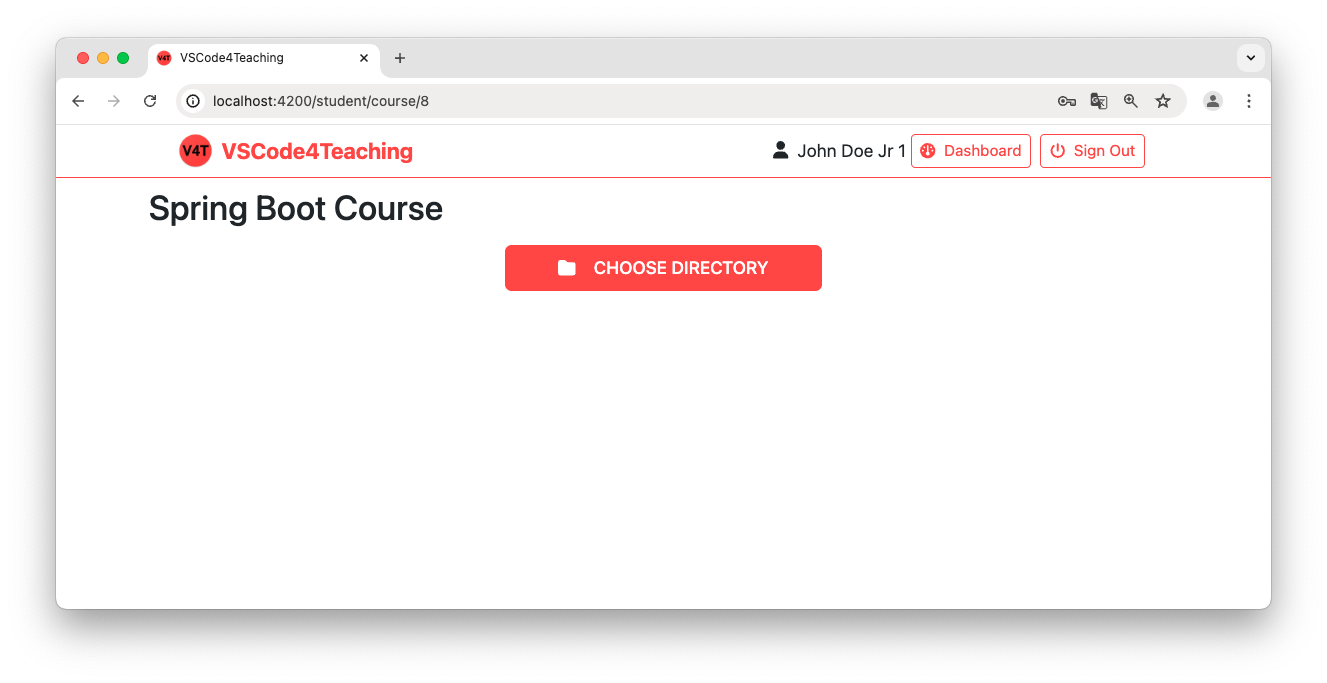
\includegraphics[width=\textwidth]{imagenes/utilizadas/4-3-implementacion/rf9-1.png}
    \caption{Situación inicial de los estudiantes al acceder al detalle de un curso y antes de elegir un directorio local.}
    \label{fig:reqf9-1}
\end{figure}

Una vez escogido el directorio, se muestra a los estudiantes el detalle de los ejercicios asociados al curso, sepárandolos en distintos paneles según su estado de ejecución: los ejercicios en progreso se sitúan en la parte superior, ubicando debajo los ejercicios no comenzados y los finalizados, tal como se refleja en la \referenciaFigura{fig:reqf9-2}. Esta ilustración permite apreciar que el estudiante tiene dos ejercicios pendientes de comenzar (``Exercise 2'' y ``Exercise 5''), ubicados dentro del panel sombreado en rojo con título ``Not started'' (no comenzado) y, además, ha finalizado un ejercicio (``Exercise 3'') que aparece dentro del panel sombreado en verde con título ``Finished'' (finalizado). A estos se suman dos ejercicios dentro del panel amarillo con título ``In progress'' (en progreso), que el estudiante podrá descargar o empezar a sincronizar, posibilidades implementadas en el requisito \referenciaConTT{subsec:rf10}{RF-10}.

\begin{figure}[ht]
    \centering
    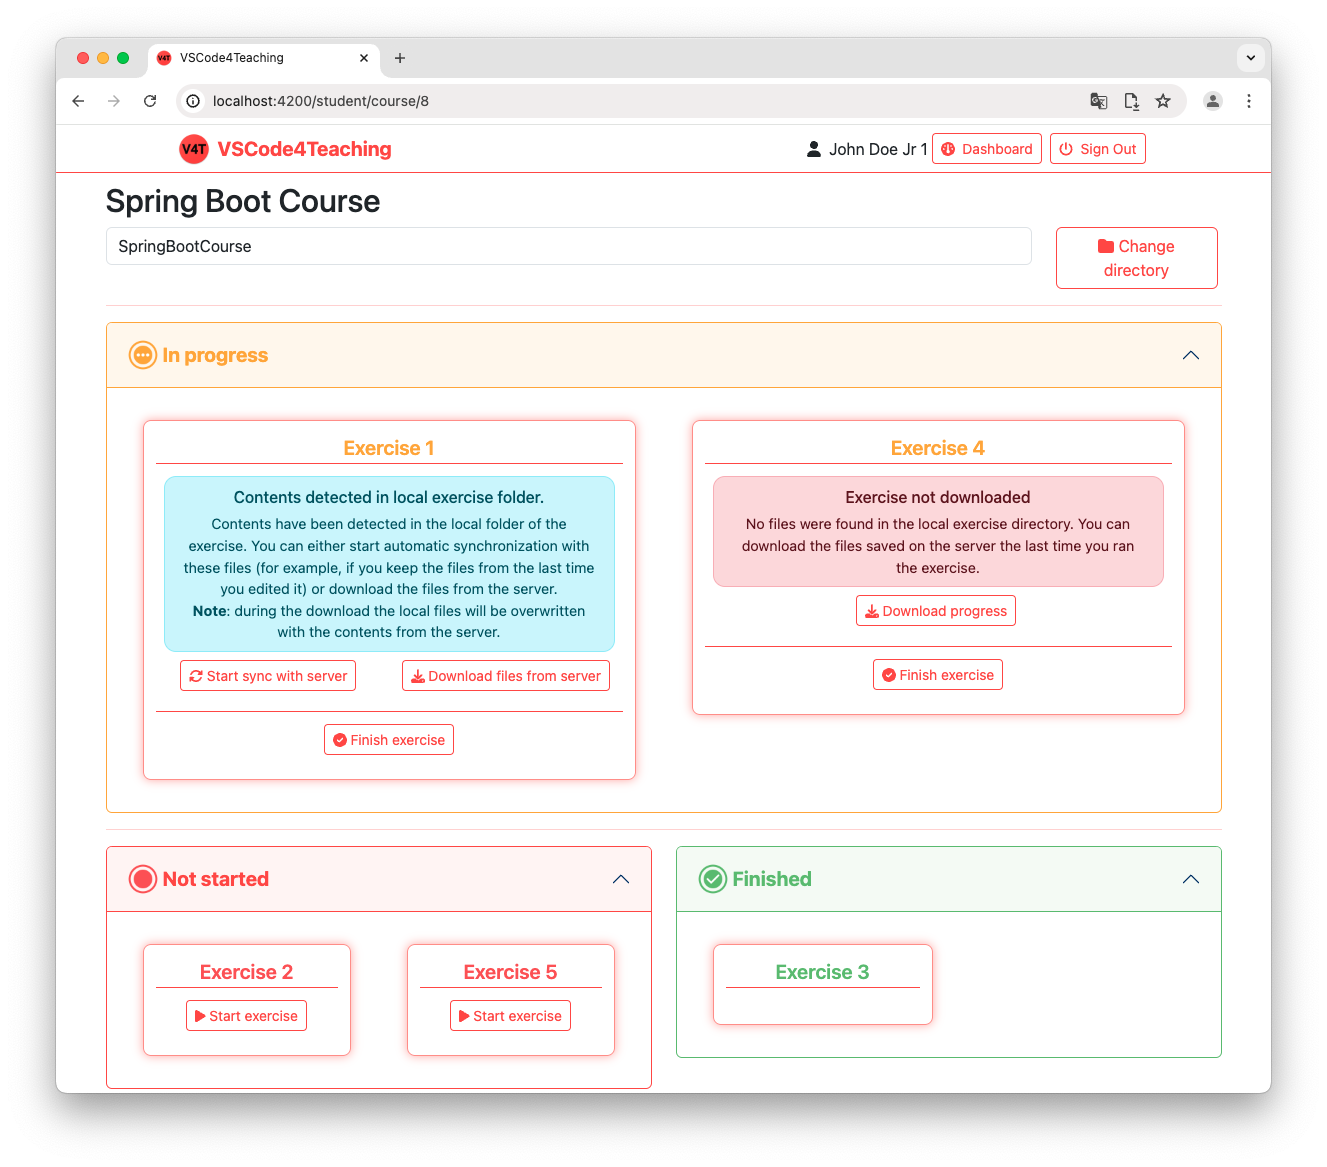
\includegraphics[width=\textwidth]{imagenes/utilizadas/4-3-implementacion/rf9-2.png}
    \caption{Visualización detallada de un curso matriculado por un estudiante con ejercicios ubicados en distintos paneles según su estado.}
    \label{fig:reqf9-2}
\end{figure}
